\documentclass[openany]{ctexbook}
\usepackage{lmodern}
\usepackage{amssymb,amsmath}
\usepackage{ifxetex,ifluatex}
\usepackage{fixltx2e} % provides \textsubscript
\ifnum 0\ifxetex 1\fi\ifluatex 1\fi=0 % if pdftex
  \usepackage[T1]{fontenc}
  \usepackage[utf8]{inputenc}
\else % if luatex or xelatex
  \ifxetex
    \usepackage{xltxtra,xunicode}
  \else
    \usepackage{fontspec}
  \fi
  \defaultfontfeatures{Ligatures=TeX,Scale=MatchLowercase}
\fi
% use upquote if available, for straight quotes in verbatim environments
\IfFileExists{upquote.sty}{\usepackage{upquote}}{}
% use microtype if available
\IfFileExists{microtype.sty}{%
\usepackage{microtype}
\UseMicrotypeSet[protrusion]{basicmath} % disable protrusion for tt fonts
}{}
\usepackage[b5paper,tmargin=2.5cm,bmargin=2.5cm,lmargin=3.5cm,rmargin=2.5cm]{geometry}
\usepackage[unicode=true]{hyperref}
\hypersetup{
            pdftitle={Guitar bookdown},
            pdfauthor={大鹏},
            pdfborder={0 0 0},
            breaklinks=true}
\urlstyle{same}  % don't use monospace font for urls
\usepackage{color}
\usepackage{fancyvrb}
\newcommand{\VerbBar}{|}
\newcommand{\VERB}{\Verb[commandchars=\\\{\}]}
\DefineVerbatimEnvironment{Highlighting}{Verbatim}{commandchars=\\\{\}}
% Add ',fontsize=\small' for more characters per line
\usepackage{framed}
\definecolor{shadecolor}{RGB}{248,248,248}
\newenvironment{Shaded}{\begin{snugshade}}{\end{snugshade}}
\newcommand{\KeywordTok}[1]{\textcolor[rgb]{0.13,0.29,0.53}{\textbf{{#1}}}}
\newcommand{\DataTypeTok}[1]{\textcolor[rgb]{0.13,0.29,0.53}{{#1}}}
\newcommand{\DecValTok}[1]{\textcolor[rgb]{0.00,0.00,0.81}{{#1}}}
\newcommand{\BaseNTok}[1]{\textcolor[rgb]{0.00,0.00,0.81}{{#1}}}
\newcommand{\FloatTok}[1]{\textcolor[rgb]{0.00,0.00,0.81}{{#1}}}
\newcommand{\ConstantTok}[1]{\textcolor[rgb]{0.00,0.00,0.00}{{#1}}}
\newcommand{\CharTok}[1]{\textcolor[rgb]{0.31,0.60,0.02}{{#1}}}
\newcommand{\SpecialCharTok}[1]{\textcolor[rgb]{0.00,0.00,0.00}{{#1}}}
\newcommand{\StringTok}[1]{\textcolor[rgb]{0.31,0.60,0.02}{{#1}}}
\newcommand{\VerbatimStringTok}[1]{\textcolor[rgb]{0.31,0.60,0.02}{{#1}}}
\newcommand{\SpecialStringTok}[1]{\textcolor[rgb]{0.31,0.60,0.02}{{#1}}}
\newcommand{\ImportTok}[1]{{#1}}
\newcommand{\CommentTok}[1]{\textcolor[rgb]{0.56,0.35,0.01}{\textit{{#1}}}}
\newcommand{\DocumentationTok}[1]{\textcolor[rgb]{0.56,0.35,0.01}{\textbf{\textit{{#1}}}}}
\newcommand{\AnnotationTok}[1]{\textcolor[rgb]{0.56,0.35,0.01}{\textbf{\textit{{#1}}}}}
\newcommand{\CommentVarTok}[1]{\textcolor[rgb]{0.56,0.35,0.01}{\textbf{\textit{{#1}}}}}
\newcommand{\OtherTok}[1]{\textcolor[rgb]{0.56,0.35,0.01}{{#1}}}
\newcommand{\FunctionTok}[1]{\textcolor[rgb]{0.00,0.00,0.00}{{#1}}}
\newcommand{\VariableTok}[1]{\textcolor[rgb]{0.00,0.00,0.00}{{#1}}}
\newcommand{\ControlFlowTok}[1]{\textcolor[rgb]{0.13,0.29,0.53}{\textbf{{#1}}}}
\newcommand{\OperatorTok}[1]{\textcolor[rgb]{0.81,0.36,0.00}{\textbf{{#1}}}}
\newcommand{\BuiltInTok}[1]{{#1}}
\newcommand{\ExtensionTok}[1]{{#1}}
\newcommand{\PreprocessorTok}[1]{\textcolor[rgb]{0.56,0.35,0.01}{\textit{{#1}}}}
\newcommand{\AttributeTok}[1]{\textcolor[rgb]{0.77,0.63,0.00}{{#1}}}
\newcommand{\RegionMarkerTok}[1]{{#1}}
\newcommand{\InformationTok}[1]{\textcolor[rgb]{0.56,0.35,0.01}{\textbf{\textit{{#1}}}}}
\newcommand{\WarningTok}[1]{\textcolor[rgb]{0.56,0.35,0.01}{\textbf{\textit{{#1}}}}}
\newcommand{\AlertTok}[1]{\textcolor[rgb]{0.94,0.16,0.16}{{#1}}}
\newcommand{\ErrorTok}[1]{\textcolor[rgb]{0.64,0.00,0.00}{\textbf{{#1}}}}
\newcommand{\NormalTok}[1]{{#1}}
\usepackage{longtable,booktabs}
% Fix footnotes in tables (requires footnote package)
\IfFileExists{footnote.sty}{\usepackage{footnote}\makesavenoteenv{long table}}{}
\usepackage{graphicx,grffile}
\makeatletter
\def\maxwidth{\ifdim\Gin@nat@width>\linewidth\linewidth\else\Gin@nat@width\fi}
\def\maxheight{\ifdim\Gin@nat@height>\textheight\textheight\else\Gin@nat@height\fi}
\makeatother
% Scale images if necessary, so that they will not overflow the page
% margins by default, and it is still possible to overwrite the defaults
% using explicit options in \includegraphics[width, height, ...]{}
\setkeys{Gin}{width=\maxwidth,height=\maxheight,keepaspectratio}
\IfFileExists{parskip.sty}{%
\usepackage{parskip}
}{% else
\setlength{\parindent}{0pt}
\setlength{\parskip}{6pt plus 2pt minus 1pt}
}
\setlength{\emergencystretch}{3em}  % prevent overfull lines
\providecommand{\tightlist}{%
  \setlength{\itemsep}{0pt}\setlength{\parskip}{0pt}}
\setcounter{secnumdepth}{5}
% Redefines (sub)paragraphs to behave more like sections
\ifx\paragraph\undefined\else
\let\oldparagraph\paragraph
\renewcommand{\paragraph}[1]{\oldparagraph{#1}\mbox{}}
\fi
\ifx\subparagraph\undefined\else
\let\oldsubparagraph\subparagraph
\renewcommand{\subparagraph}[1]{\oldsubparagraph{#1}\mbox{}}
\fi

% set default figure placement to htbp
\makeatletter
\def\fps@figure{htbp}
\makeatother

\usepackage{booktabs}
\usepackage{longtable}

\usepackage{framed,color}
\definecolor{shadecolor}{RGB}{248,248,248}

\renewcommand{\textfraction}{0.05}
\renewcommand{\topfraction}{0.8}
\renewcommand{\bottomfraction}{0.8}
\renewcommand{\floatpagefraction}{0.75}

\let\oldhref\href
\renewcommand{\href}[2]{#2\footnote{\url{#1}}}

\makeatletter
\newenvironment{kframe}{%
\medskip{}
\setlength{\fboxsep}{.8em}
 \def\at@end@of@kframe{}%
 \ifinner\ifhmode%
  \def\at@end@of@kframe{\end{minipage}}%
  \begin{minipage}{\columnwidth}%
 \fi\fi%
 \def\FrameCommand##1{\hskip\@totalleftmargin \hskip-\fboxsep
 \colorbox{shadecolor}{##1}\hskip-\fboxsep
     % There is no \\@totalrightmargin, so:
     \hskip-\linewidth \hskip-\@totalleftmargin \hskip\columnwidth}%
 \MakeFramed {\advance\hsize-\width
   \@totalleftmargin\z@ \linewidth\hsize
   \@setminipage}}%
 {\par\unskip\endMakeFramed%
 \at@end@of@kframe}
\makeatother


\usepackage{makeidx}
\makeindex

\urlstyle{tt}

\usepackage{amsthm}
\makeatletter
\def\thm@space@setup{%
  \thm@preskip=8pt plus 2pt minus 4pt
  \thm@postskip=\thm@preskip
}
\makeatother


\usepackage{xunicode}
\usepackage{fontspec}
\defaultfontfeatures{Mapping=tex-text}
\setmainfont{Microsoft YaHei}


%\usepackage{geometry}
%\setlength{\parindent}{0pt}
%\setlength{\textwidth}{7.2in}

\usepackage{gchords}

\newcommand\mychords{
\def\chordsize{1.6mm}   % distance between two frets (and two strings)
\font\fingerfont=cmr5  % font used for numbering fingers
\font\namefont=cmr10    % font used for labeling of the chord
\font\fretposfont=cmr7  % font used for the fret position marker
\def\dampsymbol{{\tiny$\scriptstyle\times$}} %  `damp this string' marker
}

\renewcommand\yoff{3}
\renewcommand\fingsiz{1.6}

% upchord
\newcommand{\AsevenMaj}{\upchord{\chord{t}{x,n,p2,p1,p2,n}{A7+}}}
\newcommand{\Aseven}{\upchord{\chord{t}{x,n,p2,n,p2,n}{A7}}}
\newcommand{\A}{\upchord{\chord{t}{x,n,p2,p2,p2,n}{A}}}
\newcommand{\Am}{\upchord{\chord{t}{n,n,p2,p2,p1,n}{Am}}}
\newcommand{\Amfive}{\upchord{\chord{{5~}}{p1,p3,p3,p1,p1,p1}{Am(5)}}}
\newcommand{\Bb}{\upchord{\chord{t}{f1p1,f1p1,p3,p3,p3,f1p1}{$^b$B}}}
\newcommand{\BmseveN}{\upchord{\chord{t}{x,p2,p4,p3,p3,p2}{Bm7+}}}
\newcommand{\BmsevenA}{\upchord{\chord{t}{x,n,p4,p4,p3,n}{Bm/A}}}
\newcommand{\Bmseven}{\upchord{\chord{t}{x,p2,p4,p2,p3,p2}{Bm7}}}
\newcommand{\Bm}{\upchord{\chord{t}{x,p2,p4,p4,p3,p2}{Bm}}}
\newcommand{\BM}{\upchord{\chord{t}{f1p2,f1p2,p4,p4,p4,f1p2}{B}}}
\newcommand{\Bseven}{\upchord{\chord{t}{x,f1p2,p4,f1p2,p4,f1p2,}{B7}}}
\newcommand{\BMseven}{\upchord{\chord{t}{n,p2,p1,p2,n,p2}{B7}}}
\newcommand{\BsevenBasDs}{\upchord{\chord{t}{x,x,p1,p2,n,p2}{B7/D\#}}}
\newcommand{\CM}{\upchord{\chord{t}{n,p3,p2,n,p1,n}{C}}}
\newcommand{\CssevenLight}{\upchord{\chord{t}{x,p4,p3,p4,p2,x}{C\#7}}}
\newcommand{\Csthree}{\upchord{\chord{{4~}}{f1p1,f1p1,p3,p3,p3,f1p1}{$^\#$C}}}
\newcommand{\Cthree}{\upchord{\chord{{3~}}{f1p1,f1p1,p3,p3,p3,f1p1}{C(3)}}}
\newcommand{\Cseven}{\upchord{\chord{t}{n,p3,p2,p3,p1,n}{C7}}}
\newcommand{\Cm}{\upchord{\chord{t}{f1p3,f1p3,p5,p5,p4,f1p3}{Cm}}}
\newcommand{\Csm}{\upchord{\chord{{4~}}{f1p1,f1p1,p3,p3,p2,f1p1}{\#Cm}}}
\newcommand{\DmBasB}{\upchord{\chord{t}{x,p2,p3,p2,p3,x}{Dm/B}}}
\newcommand{\DseveN}{\upchord{\chord{t}{x,x,n,p2,p2,p2}{D7+}}}
\newcommand{\Dseven}{\upchord{\chord{t}{x,x,n,p2,p1,p2}{D7}}}
\newcommand{\Dsix}{\upchord{\chord{t}{x,x,n,p2,n,p2}{D6}}}
\newcommand{\D}{\upchord{\chord{t}{x,x,n,p2,p3,p2}{D}}}
\newcommand{\Dm}{\upchord{\chord{t}{x,x,n,p2,p3,p1}{Dm}}}
\newcommand{\Eb}{\upchord{\chord{{6~}}{f1p1,f1p1,p3,p3,p3,f1p1}{$^b$E}}}
\newcommand{\E}{\upchord{\chord{t}{n,p2,p2,p1,n,n}{E}}}
\newcommand{\Eseven}{\upchord{\chord{{7~}}{f1p1,f1p1,p3,p3,p3,f1p1}{E(7)}}}
\newcommand{\EseveNNine}{\upchord{\chord{t}{n,f1p2,f1p2,p4,p3,f1p2,}{E79}}}
\newcommand{\EseveN}{\upchord{\chord{t}{n,p2,p2,p4,p3,p4}{E7}}}
\newcommand{\EsevenFour}{\upchord{\chord{t}{n,p2,p2,p4,p3,p5}{E7,11}}}
\newcommand{\Em}{\upchord{\chord{t}{n,p2,p2,n,n,n}{Em}}}
\newcommand{\F}{\upchord{\chord{t}{f1p1,p3,p3,p2,f1p1,f1p1}{F}}}
\newcommand{\Fs}{\upchord{\chord{t}{f2p2,p4,p4,p3,f1p2,f1p2}{F\#}}}
\newcommand{\Fsmin}{\upchord{\chord{t}{f1p2,p4,p4,f1p2,f1p2,f1p2,}{F\#m}}}
\newcommand{\FsminLight}{\upchord{\chord{t}{x,x,f3p4,f1p2,f1p2,f1p2,}{F\#m}}}
\newcommand{\FsminBasSeveN}{\upchord{\chord{t}{x,x,f3p3,f1p2,f1p2,f1p2,}{F\#m/E\#}}}
\newcommand{\FsminBasSeven}{\upchord{\chord{t}{x,x,f2p2,f1p2,f1p2,f1p2,}{F\#m/E}}}
\newcommand{\FsminSeven}{\upchord{\chord{t}{f1p2,p4,p4,f1p2,p5,f1p2,}{F\#7m}}}
\newcommand{\GM}{\upchord{\chord{t}{p3,p2,n,n,n,p3}{G}}}
\newcommand{\Gsminseven}{\upchord{\chord{t}{f2p4,x,f4p4,f4p4,f4p4,f4p4,}{G\#7}}}
\newcommand{\Gthree}{\upchord{\chord{t}{f1p3,p5,p5,p4,f1p3,f1p3}{G(3)}}}
\newcommand{\Gm}{\upchord{\chord{{3~}}{f1p1,p3,p3,f1p1,f1p1,f1p1}{Gm}}}
\newcommand{\Gsm}{\upchord{\chord{{4~}}{f1p1,p3,p3,f1p1,f1p1,f1p1}{\#Gm}}}
\newcommand{\Gseven}{\upchord{\chord{t}{p3,p2,n,n,n,p1}{G7}}}

%inline 
\newcommand{\iAsevenMaj}{\chord{t}{x,n,p2,p1,p2,n}{A7+}}
\newcommand{\iAseven}{\chord{t}{x,n,p2,n,p2,n}{A7}}
\newcommand{\iA}{\chord{t}{x,n,p2,p2,p2,n}{A}}
\newcommand{\iAm}{\chord{t}{n,n,p2,p2,p1,n}{Am}}
\newcommand{\iAmfive}{\chord{{5~}}{p1,p3,p3,p1,p1,p1}{Am(5)}}
\newcommand{\iBb}{\chord{t}{f1p1,f1p1,p3,p3,p3,f1p1}{$^b$B}}
\newcommand{\iBmseveN}{\chord{t}{x,p2,p4,p3,p3,p2}{Bm7+}}
\newcommand{\iBmsevenA}{\chord{t}{x,n,p4,p4,p3,n}{Bm/A}}
\newcommand{\iBmseven}{\chord{t}{x,p2,p4,p2,p3,p2}{Bm7}}
\newcommand{\iBm}{\chord{t}{x,p2,p4,p4,p3,p2}{Bm}}
\newcommand{\iBM}{\chord{t}{f1p2,f1p2,p4,p4,p4,f1p2}{B}}
\newcommand{\iBseven}{\chord{t}{x,f1p2,p4,f1p2,p4,f1p2,}{B7}}
\newcommand{\iBMseven}{\chord{t}{n,p2,p1,p2,n,p2}{B7}}
\newcommand{\iBsevenBasDs}{\chord{t}{x,x,p1,p2,n,p2}{B7/D\#}}
\newcommand{\iCM}{\chord{t}{n,p3,p2,n,p1,n}{C}}
\newcommand{\iCssevenLight}{\chord{t}{x,p4,p3,p4,p2,x}{C\#7}}
\newcommand{\iCsthree}{\chord{{4~}}{f1p1,f1p1,p3,p3,p3,f1p1}{$^\#$C}}
\newcommand{\iCthree}{\chord{{3~}}{f1p1,f1p1,p3,p3,p3,f1p1}{C(3)}}
\newcommand{\iCseven}{\chord{t}{n,p3,p2,p3,p1,n}{C7}}
\newcommand{\iCm}{\chord{t}{f1p3,f1p3,p5,p5,p4,f1p3}{Cm}}
\newcommand{\iCsm}{\chord{{4~}}{f1p1,f1p1,p3,p3,p2,f1p1}{\#Cm}}
\newcommand{\iDmBasB}{\chord{t}{x,p2,p3,p2,p3,x}{Dm/B}}
\newcommand{\iDseveN}{\chord{t}{x,x,n,p2,p2,p2}{D7+}}
\newcommand{\iDseven}{\chord{t}{x,x,n,p2,p1,p2}{D7}}
\newcommand{\iDsix}{\chord{t}{x,x,n,p2,n,p2}{D6}}
\newcommand{\iD}{\chord{t}{x,x,n,p2,p3,p2}{D}}
\newcommand{\iDm}{\chord{t}{x,x,n,p2,p3,p1}{Dm}}
\newcommand{\iEb}{\chord{{6~}}{f1p1,f1p1,p3,p3,p3,f1p1}{$^b$E}}
\newcommand{\iE}{\chord{t}{n,p2,p2,p1,n,n}{E}}
\newcommand{\iEseven}{\chord{{7~}}{f1p1,f1p1,p3,p3,p3,f1p1}{E(7)}}
\newcommand{\iEseveNNine}{\chord{t}{n,f1p2,f1p2,p4,p3,f1p2,}{E79}}
\newcommand{\iEseveN}{\chord{t}{n,p2,p2,p4,p3,p4}{E7}}
\newcommand{\iEsevenFour}{\chord{t}{n,p2,p2,p4,p3,p5}{E7,11}}
\newcommand{\iEm}{\chord{t}{n,p2,p2,n,n,n}{Em}}
\newcommand{\iF}{\chord{t}{f1p1,p3,p3,p2,f1p1,f1p1}{F}}
\newcommand{\iFs}{\chord{t}{f2p2,p4,p4,p3,f1p2,f1p2}{F\#}}
\newcommand{\iFsmin}{\chord{t}{f1p2,p4,p4,f1p2,f1p2,f1p2,}{F\#m}}
\newcommand{\iFsminLight}{\chord{t}{x,x,f3p4,f1p2,f1p2,f1p2,}{F\#m}}
\newcommand{\iFsminBasSeveN}{\chord{t}{x,x,f3p3,f1p2,f1p2,f1p2,}{F\#m/E\#}}
\newcommand{\iFsminBasSeven}{\chord{t}{x,x,f2p2,f1p2,f1p2,f1p2,}{F\#m/E}}
\newcommand{\iFsminSeven}{\chord{t}{f1p2,p4,p4,f1p2,p5,f1p2,}{F\#7m}}
\newcommand{\iGM}{\chord{t}{p3,p2,n,n,n,p3}{G}}
\newcommand{\iGsminseven}{\chord{t}{f2p4,x,f4p4,f4p4,f4p4,f4p4,}{G\#7}}
\newcommand{\iGthree}{\chord{t}{f1p3,p5,p5,p4,f1p3,f1p3}{G(3)}}
\newcommand{\iGm}{\chord{{3~}}{f1p1,p3,p3,f1p1,f1p1,f1p1}{Gm}}
\newcommand{\iGsm}{\chord{{4~}}{f1p1,p3,p3,f1p1,f1p1,f1p1}{\#Gm}}
\frontmatter

\title{Guitar bookdown}
\author{大鹏}
\date{2017-04-07}

\usepackage{amsthm}
\newtheorem{theorem}{Theorem}[chapter]
\newtheorem{lemma}{Lemma}[chapter]
\theoremstyle{definition}
\newtheorem{definition}{Definition}[chapter]
\newtheorem{corollary}{Corollary}[chapter]
\newtheorem{proposition}{Proposition}[chapter]
\theoremstyle{definition}
\newtheorem{example}{Example}[chapter]
\theoremstyle{remark}
\newtheorem*{remark}{Remark}
\begin{document}
\maketitle

\thispagestyle{empty}

\setlength{\abovedisplayskip}{-5pt}
\setlength{\abovedisplayshortskip}{-5pt}

%\mychords

{
\setcounter{tocdepth}{1}
\tableofcontents
}
\chapter*{前言}\label{front}
\addcontentsline{toc}{chapter}{前言}

最真的梦,就是用R语言的bookdown把R代码、作图、数据分析和吉他谱弄到一起。

啥?弄到一起有什么用?

呃\ldots{}\ldots{}容我清清脑子想一想\ldots{}\ldots{}

\begin{quote}
--- 大鹏
\end{quote}

\begin{Shaded}
\begin{Highlighting}[]
 \KeywordTok{persp}\NormalTok{(x, y, z, }\DataTypeTok{theta =} \DecValTok{120}\NormalTok{, }\DataTypeTok{phi =} \DecValTok{15}\NormalTok{, }\DataTypeTok{scale =} \OtherTok{FALSE}\NormalTok{, }
       \DataTypeTok{axes =} \OtherTok{FALSE}\NormalTok{)}
\end{Highlighting}
\end{Shaded}

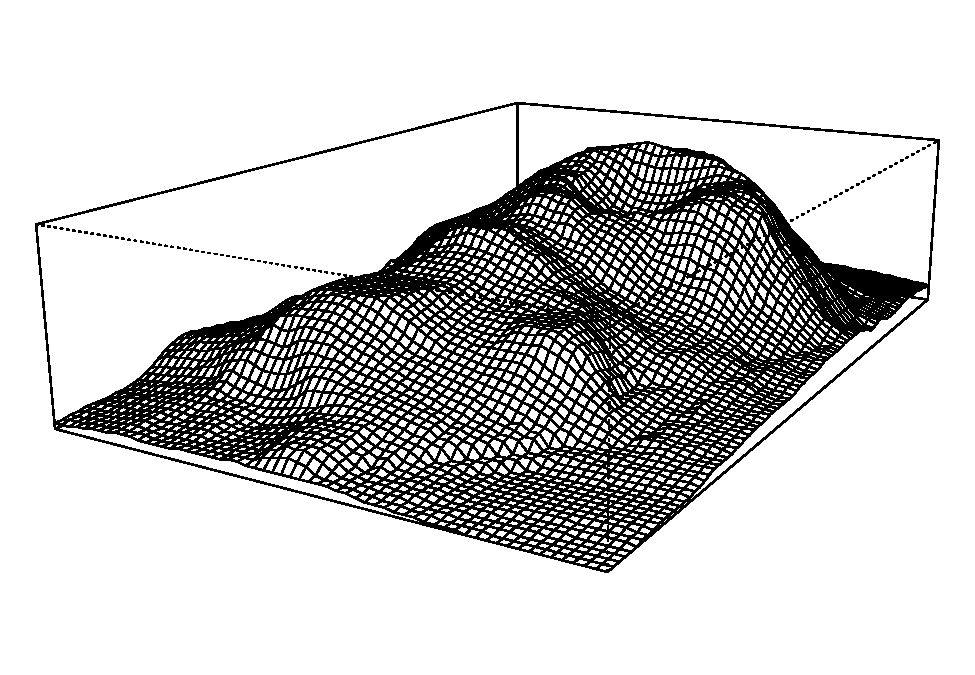
\includegraphics[width=0.6\linewidth]{bdguitar_files/figure-latex/unnamed-chunk-1-1}

终会有\Am 一天 把心愿\Dm 完成 

带着你\F 飞奔\GM 找永\Cm 恒\Csthree \Cthree  

\[\int_0^\infty e^{-x^2} dx=\frac{\sqrt{\pi}}{2}\]

本书的吉他谱,在网页上看不见,只有点击下载pdf才能看见哦。

\mainmatter

\part{用R bookdown记吉他谱}\label{method}

\chapter*{简介}\label{intro}
\addcontentsline{toc}{chapter}{简介}

前情提要:

\begin{itemize}
\tightlist
\item
  \href{http://dapengde.com/archives/19122}{用 R 语言的 bookdown 写书}
\item
  \href{http://dapengde.com/archives/19150}{用 R 语言的 bookdown 写诗集}
\item
  \href{http://dapengde.com/archives/19190}{用 R 语言的 bookdown
  写学术论文}
\item
  \href{http://dapengde.com/archives/19141}{R 语言 bookdown
  快速入门和语法速查}
\end{itemize}

本篇说说如何用 R 语言的 bookdown
写吉他谱。别拦着我,让我陷进bookdown的怀抱里爽死吧。

中国的民谣吉他伴奏谱常见的一般是六线谱,格式是这样的:

\begin{figure}[htbp]
\centering
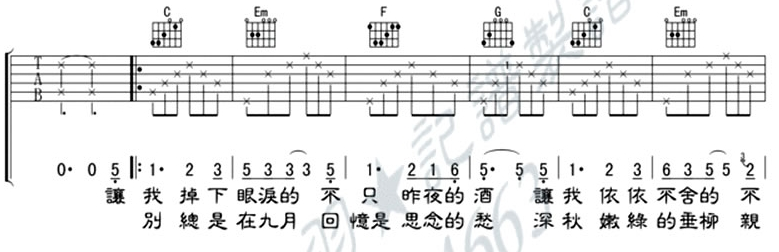
\includegraphics{images/chengdu1-.jpg}
\caption{}
\end{figure}

\begin{itemize}
\tightlist
\item
  第一行是和弦谱,包括和弦名称和左手按琴弦的指法图;
\item
  第二行是六线谱,右手拨弦的方式(当然也夹杂左手按和弦外音的变化);
\item
  第三行是歌曲旋律的简谱;
\item
  第四行是歌词。
\end{itemize}

前两行的和弦谱和六线谱在录入时需要专业软件,太麻烦;歌曲旋律一般是跟着原唱学,基本用不着;歌词最容易录入。由于和弦谱最为重要,任何乐器伴奏都用得着,为了省事儿,上图可以只保留和弦名称和歌词,简化为文字谱:

\begin{verbatim}
  C    Em     F     G    C    Em
让我掉下眼泪的不只昨夜的酒,让我依依不舍的不……
\end{verbatim}

文字谱的好处是用不着任何专业软件,录入很方便。但是,这比较坑菜鸟。想不起来\texttt{Em}和弦的指法该怎么办?\texttt{Em}还好办,看见个\texttt{G\#7sus4},我崩溃了,自认水平不行,乖乖翻和弦字典去。如果标注了指法图------

让\CM 我掉下\Em 眼泪的 不\F 只昨夜的\GM 酒 让\CM 我依依\Em 不\ldots{}\ldots{}

还是更方便一些,吉他和钢琴都可以用。我觉得等我老得掉光牙齿的时候,估计连C和弦的指法都忘光了,给孙子连个《成都》都唱不成,这时候指法图就有用了。

以前我玩过\href{http://dapengde.com/archives/18230}{LaTeX输入指法图}的游戏。由于对LaTeX心怀恐惧,这个游戏没敢多玩。现在有了R语言的bookdown来取代LaTeX,自然想把这个游戏拿回来找找年轻的感觉。

这个主意早就有了,原以为会很麻烦(恐惧心理),一直没行动。昨天在送大娃和接二娃之间空出半个小时,鼓捣了一下,居然鼓捣出来了上面那个样子。其实很简单:用
bookdown 的壳,LaTeX的核。上面那句歌词,录入的文字是这样的:

\begin{verbatim}
让\CM 我掉下\Em 眼泪的 不\F 只昨夜的\GM 酒 让\CM 我依依\Em 不舍的 不……
\end{verbatim}

我打算以后陆陆续续把喜欢的歌弄成一本书,并且把bookdown录入吉他谱的源代码在\href{https://github.com/dapengde/bookdown-guitar}{GitHub开了个bookdown-guitar的项目}。毕竟,中文的对齐不太完美,看看有没有高手来帮帮我。

其实跟LaTeX里一样。那我在LaTeX里用就行了,干嘛来bookdown里用?

因为这样的话,就可以在同一本书里同时呈现R代码、作图、分析结果和吉他谱啊。

啊?把他们弄在一起有什么用?

呃\ldots{}\ldots{}这是个好问题\ldots{}\ldots{}容我清清脑子想一想\ldots{}\ldots{}听说数学领域很多理论在提出时都没啥用,后来都用上了,除了数论\ldots{}\ldots{}我不会运气跟数论一样好吧\ldots{}\ldots{}

\part{最真的梦}\label{true-dream}

\chapter*{成都}\label{cd}
\addcontentsline{toc}{chapter}{成都}

作词:赵雷,作曲:赵雷,编曲:赵雷、喜子。

前奏:\iCM

让\CM 我掉下\Em 眼泪的 不\F 只昨夜的\GM 酒 

让\CM 我依依\Em 不舍的 不\F 只你的温\GM 柔

余\Em 路还要\Am 走多久 你\F 攥着\GM 我的\CM 手

让\Em 我感到\F 为难的 是\GM 挣扎\CM 的自由

分\CM 别总是\Em 在九月 回\F 忆是思念的\GM 愁

深\CM 秋嫩绿的\Em 垂柳 亲\F 吻着我额\GM 头

在\Em 那座阴雨的\Am 小城里 我\F 从未\GM 忘记\CM 你

成\Em 都 带不\F 走的 \GM 只有\CM 你 \Cseven

和\Em 我在成都的\Am 街头走一\F 走 呜\GM 哦呜\CM 哦

直\Em 到所有的\Am 灯都熄灭\F 了也\GM 不停\CM 留

你会\F 挽着\GM 我的衣\CM 袖 我会\F 把手\GM 揣进裤\CM 兜

走\Dm 到玉林路的尽头 坐\GM 在(走过)小酒馆的门口

\chapter*{夜半歌声}\label{ybgs}
\addcontentsline{toc}{chapter}{夜半歌声}

(前奏)\chords{{\iCm} {\iAmfive} {\iCm} {\iGm} {\iDm}{\iAm}{\iBb}{\iCseven}}

只有在\F 夜深 我和你\Gm 才能 敞开灵\Dm 魂 去释放天\Am 真 \qquad \Cm  

把温柔\F  的吻 在夜半\Gm 时分 化成歌\Dm 声 \Am 依偎你心\GM 门

我祈求\Cm  星辰 月儿来\Dm 作证 用尽一\Am 生 也愿意去\Em 等

终会有\Am 一天 把心愿\Dm 完成 带着你\F  飞奔\GM  找永\Cm  恒
\qquad \Csthree  \qquad \Cthree     

\chapter*{Hallelujah}\label{hallelujah}
\addcontentsline{toc}{chapter}{Hallelujah}

I've \CM heard there was a \Am secret chord

That \CM David played, and it \Am pleased the Lord

But \F you don't really care for music, \CM do you? \GM

It \CM goes like this: The \F fourth, the \GM fifth

The \Am minor fall, the \GM major lift

The \GM baffled king com\Em -posing Halle\Am -lujah

Halle\F -lujah, Halle\CM -lujah Halle\F -lujah, Halle
\CM -lu\GM -\CM jah

Your faith was strong But you needed proof

You saw her bathing On the roof

Her beauty and the Moonlight overthrew you

She tied you to a kitchen chair

She broke your throne And she cut your hair

And from your lips She drew the Hallelujah

Hallelujah, Hallelujah, Hallelujah, Hallelujah

Maybe I've been here before

I know this room I've walked this floor

I used to live alone Before I knew you

I've seen your flag On the marble arch

Love is not a victory march

It's a cold and It's a broken Hallelujah

Hallelujah, Hallelujah, Hallelujah, Hallelujah

There was a time You let me know

What's really going on below

But now you never show It to me, do you?

I remember when I moved in, you

Your holy dark Was moving too

And every breath we drew Was Hallelujah

Hallelujah, Hallelujah Hallelujah, Hallelujah

Maybe there's a God above

And all I ever Learned from love

Was how to shoot At someone Who outdrew you

It's not a cry You can hear at night

It's not somebody Who's seen the light

It's a cold and It's a broken Hallelujah

Hallelujah, Hallelujah, Hallelujah, Hallelujah

\chapter*{附录:常用和弦指法图}\label{appendix}
\addcontentsline{toc}{chapter}{附录:常用和弦指法图}

\chords{\iAsevenMaj \iAseven \iA \iAm \iAmfive}

\chords{\iBb \iBmseveN \iBmsevenA \iBmseven \iBm \iBM \iBseven \iBMseven \iBsevenBasDs}

\chords{\iCM \iCssevenLight \iCsthree \iCthree \iCseven \iCm \iCsm}

\chords{\iDmBasB \iDseveN \iDseven \iDsix \iD \iDm}

\chords{\iEb \iE \iEseven \iEseveNNine \iEseveN \iEsevenFour \iEm}

\chords{\iF \iFs \iFsmin \iFsminLight \iFsminBasSeveN \iFsminBasSeven \iFsminSeven}

\chords{\iGM \iGsminseven \iGthree \iGm \iGsm}

\backmatter

\end{document}
